\documentclass[]{article}   
\usepackage{graphicx}
\usepackage{xcolor} 
\usepackage{subcaption}
\usepackage{wrapfig}
\usepackage[utf8]{inputenc}
\usepackage{amsmath}
\usepackage{float}
%\usepackage{todonotes} 
\usepackage{color}
\usepackage{epstopdf}
\usepackage{mdframed}
\usepackage[a4paper]{geometry}
\geometry{top=3cm,left=4cm, right=4cm}
\sloppy
\definecolor{lightgray}{gray}{0.5}
\setlength{\parindent}{0pt}
\renewcommand{\figurename}{Figura}
\newcommand{\CP}[1]{\textcolor{blue}{#1}}
%SetFonts
%Title Page
\title{Robòtica industrial i de serveis. \\ Projecte final \\ Implementació d'estructures de control utilitzant la Robotics Toolbox. }
\author{Guillem Casado, Albert Llebaria}
\date{Gener 2019}                           
\begin{document}
\maketitle
\begin{abstract}
\end{abstract}
\section{Objectius}
L'objectiu d'aquest projecte és implementar dues estructures de control per al moviment d'un robot. Aquestes són: 
\begin{itemize}
\item Controlador PD amb compensació de gravetat en l'espai d'articulacions. 
\item Control de dinàmica inversa en l'espai d'articulacions.
\end{itemize}
Per tal d'assolir-ho, s'ha de dur a terme els següents punts:
\begin{itemize}
\item Per cada estratègia de control, implementar el sistema mitjançant SIMULINK. 
\item Utilitzar la llibreria Robotic Toolbox per a la realització del projecte. 
\item Utilitzar el robot PUMA560, ja que es disposen les seves característiques (inèrcia, coriolis...) per facilitar la implementació. 
\item Proporcionar un script per configurar paràmetres com ara les constants dels controladors, configuracions inicial i final de les articulacions del robot etc.
\item Mostrar una animació del robot movent-se de posició inicial a final en cada execució del SIMULINK de cada estratègia de control. Això permet comprovar que la implementació és correcta. 
\end{itemize}
\section{Controlador PD amb compensació de gravetat en l'espai d'articulacions}
\subsection{Estudi del model teòric a implementar}
Per aquesta estructura de control, es desitja assolir una determinada configuració d'articulacions, $q_{d}$. D'aquesta manera, l'error serà $\tilde{q} = q_{d} - q$. El model del robot a controlar és $B(q)\ddot{q} + C(q, \dot{q})\dot{q} + F\dot{q} + g(q) = u$. Donada la no linealitat d'aquest, es fa ús del mètode de Lyapunov per tal de garantir que la llei de control porti al robot fins a la configuració desitjada d'una manera assimptòticament estable. La funció de Lyapunov $V(q, \dot{q})$ per aquest model és: \\
\centerline{$V(q, \dot{q}) = \frac{1}{2}\dot{q}^TB(q,\dot{q}) +  \frac{1}{2}\tilde{q}^TK_{p}\tilde{q} > 0 , \forall\dot{q},q \neq 0$ } \leavevmode \\
Si $\dot{V}(q, \dot{q}) < 0$, llavors es pot garantir l'estabilitat. La derivada de la funció de Lyapunov resulta de la següent manera: \\
\centerline{$\dot{V}(q, \dot{q})= -\dot{q}^TF(\dot{q}) + \dot{q}^T[u - g(q) - K_{p}\tilde{q}]$} \leavevmode \\
Donat que el primer terme de la derivada és sempre negatiu, una possibilitat per assegurar l'estabilitat és que el segon terme sigui zero. D'aquesta manera, es decideix que la llei de control sigui: \\
\centerline{$u = g(q) + K_{p}\tilde{q}$} \leavevmode \\
Finalment, per accelerar la convergència, s'afegeix un terme derivatiu. La llei de control final, queda doncs, expressada de la forma següent: \\
\centerline{$u = g(q) + K_{p}\tilde{q} -K_{D}\dot{q}$} \leavevmode \\
Un cop definides les equacions del sistema de control, el sistema expressat en blocs resulta com el mostrat en la figura \ref{fig:PD_block_diagram}. \\

\begin{figure}[H]
\centering
    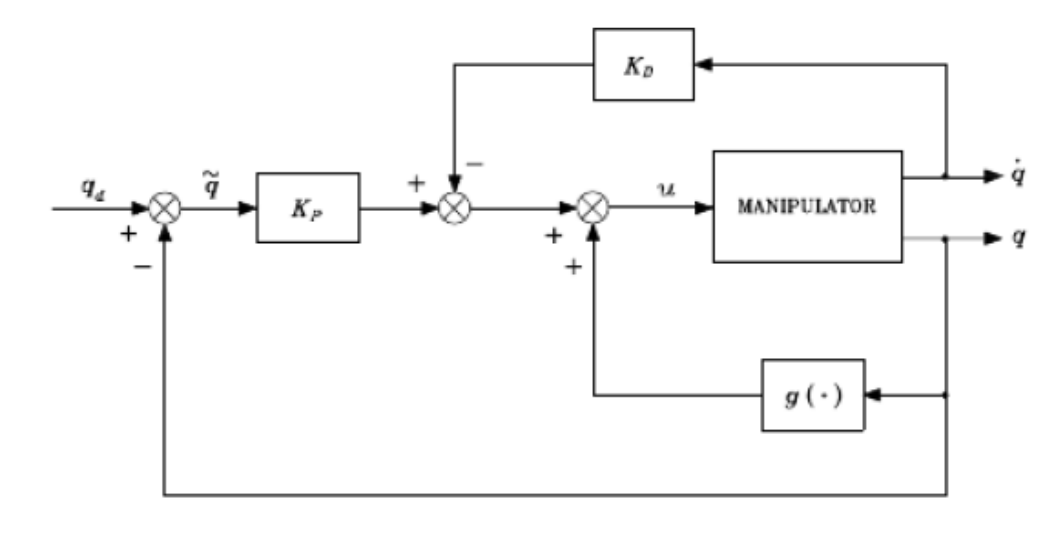
\includegraphics[width = 1\linewidth]{images/PD_gravity_compensation_Block_Diagram.png}
    \caption{Esquema de blocs del sistema.}
    \label{fig:PD_block_diagram}
\end{figure}

\subsection{Implementació del controlador amb Matlab}
Un cop definit el senyal de control i el diagrama de blocs, es procedeix a implementar-ho en el SIMULINK de Matlab. El resultat del diagrama de blocs es mostra en la figura \ref{fig:PD_simulink}. \\
\begin{figure}[H]
\centering
    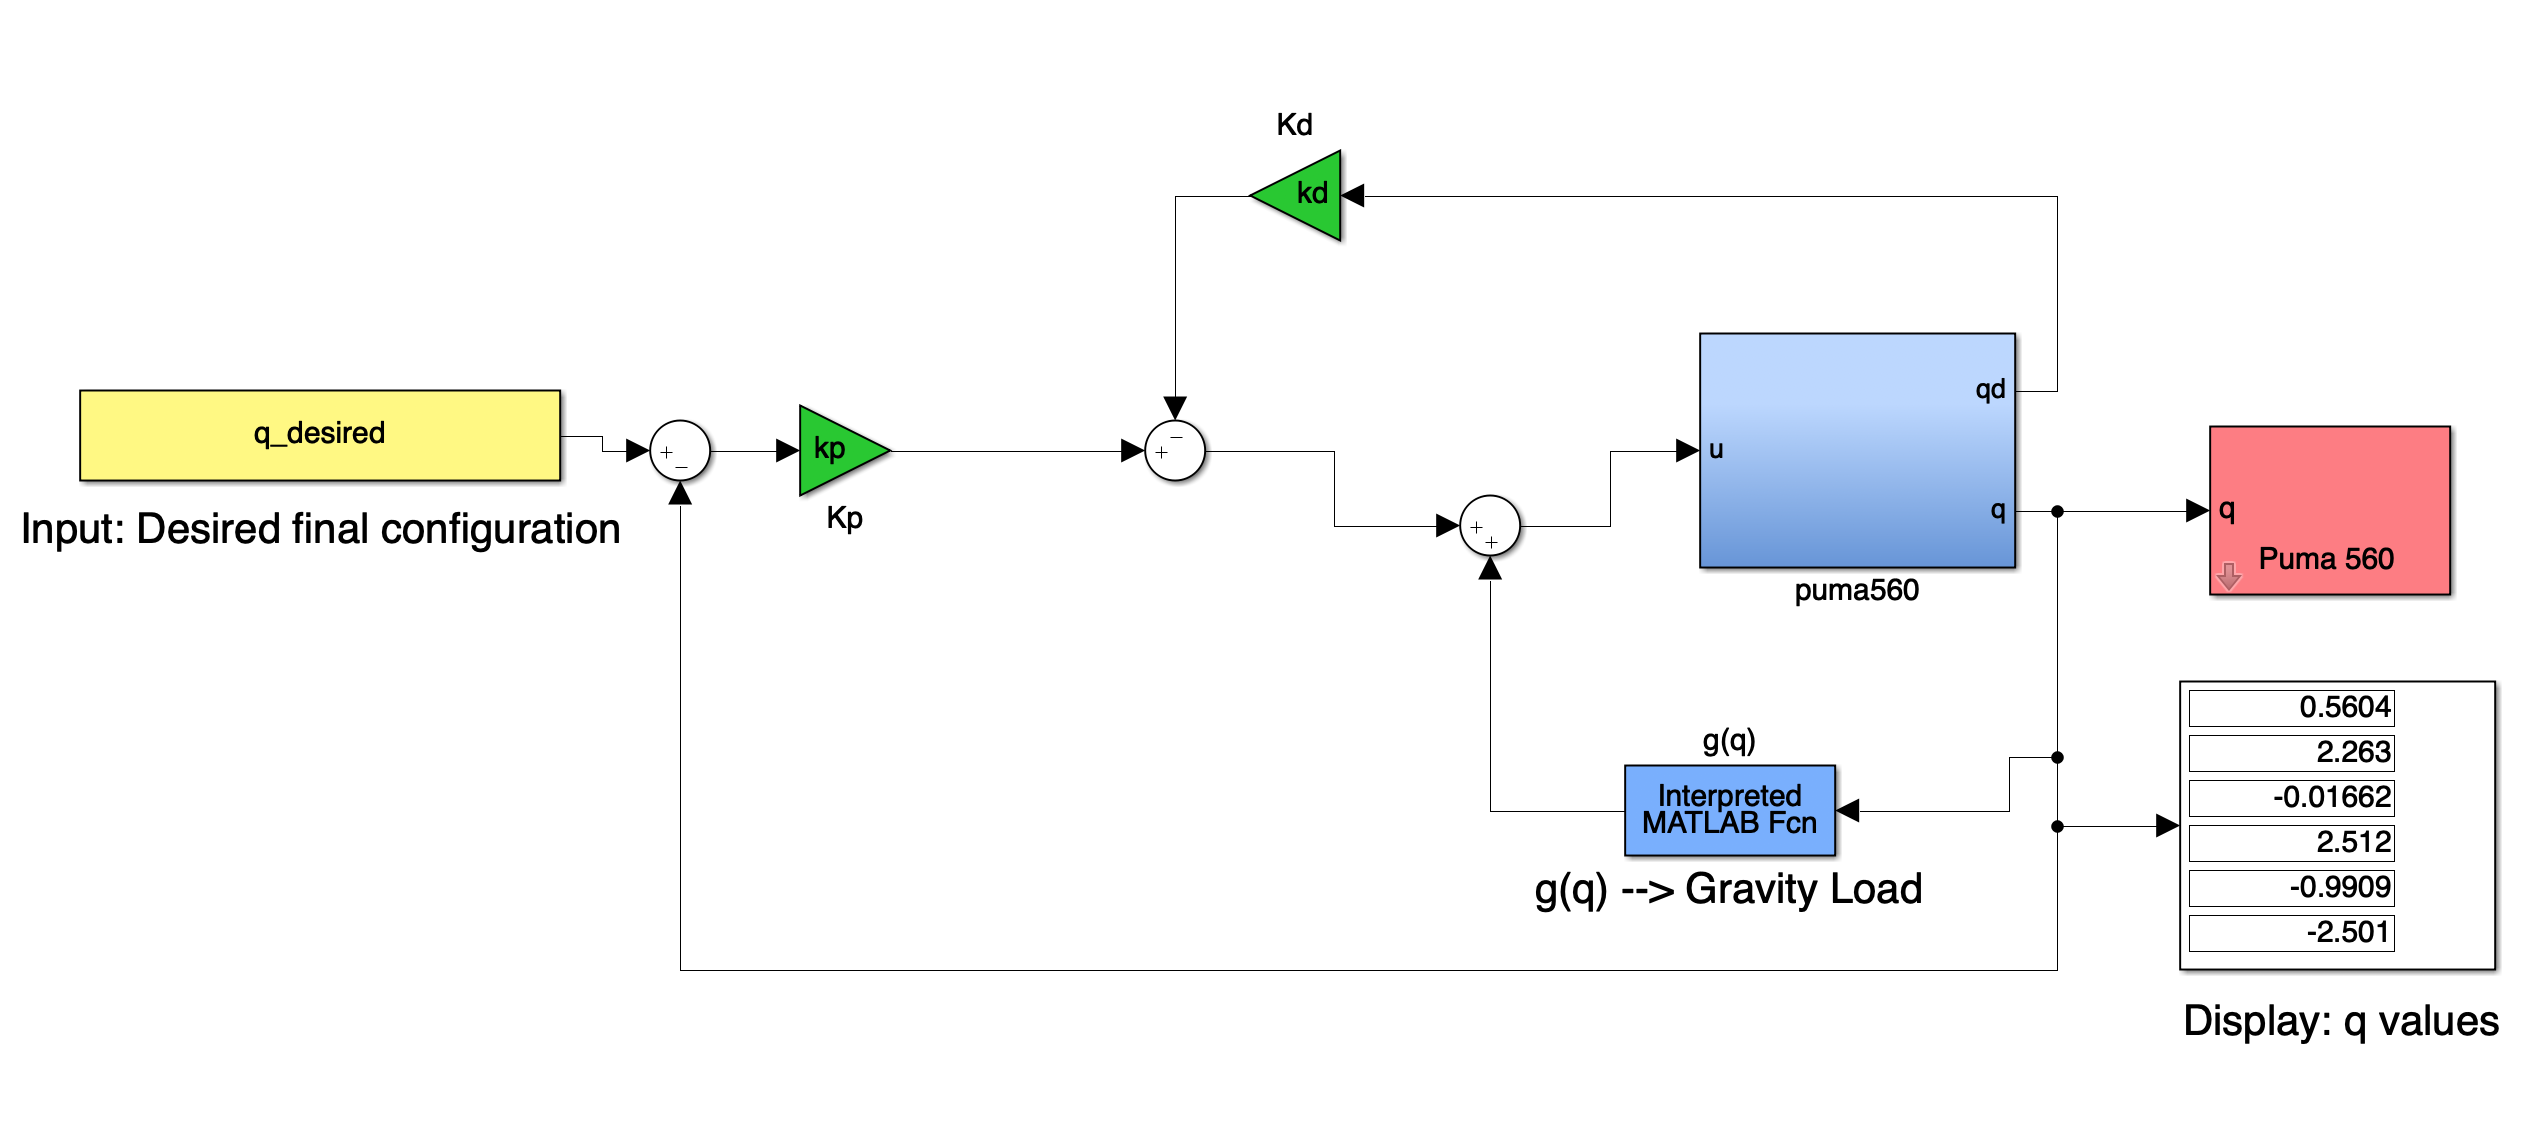
\includegraphics[width = 1\linewidth]{images/PD_gravity_compensation_Simulink.png}
    \caption{Esquema de blocs del sistema en Simulink.}
    \label{fig:PD_simulink}
\end{figure}

Els valors de $q_{d}$, $K_{p}$ i $K_{d}$ es defineixen en script ////X.m. El bloc $g(q)$ correspon a la compensació de gravetat donada una configuració d'articulacions. Donat que el PUMA560 ja disposa de totes les seves característiques, es pot obtenir el valor del bloc simplement amb la comanda



\end{document}